\question \textit{The following question is extremely difficult. Something
like this would not appear on the exam. Nonetheless, it's a fun problem to
try.}

Draw the environment diagram that results from executing the code below.

Note that using the \texttt{+} operator with two strings results in the
second string being appended to the first. For example \texttt{"C" + "S"}
concatenates the two strings into one string \texttt{"CS"}
\begin{lstlisting}[numbers=left, numberfirstline=false]
y = "y"
h = y
def y(y):
    h = "h"
    if y == h:
        return y + "i"
    y = lambda y: y(h)
    return lambda h: y(h)
y = y(y)(y)
\end{lstlisting}

\begin{solution}[2in]
\begin{center}
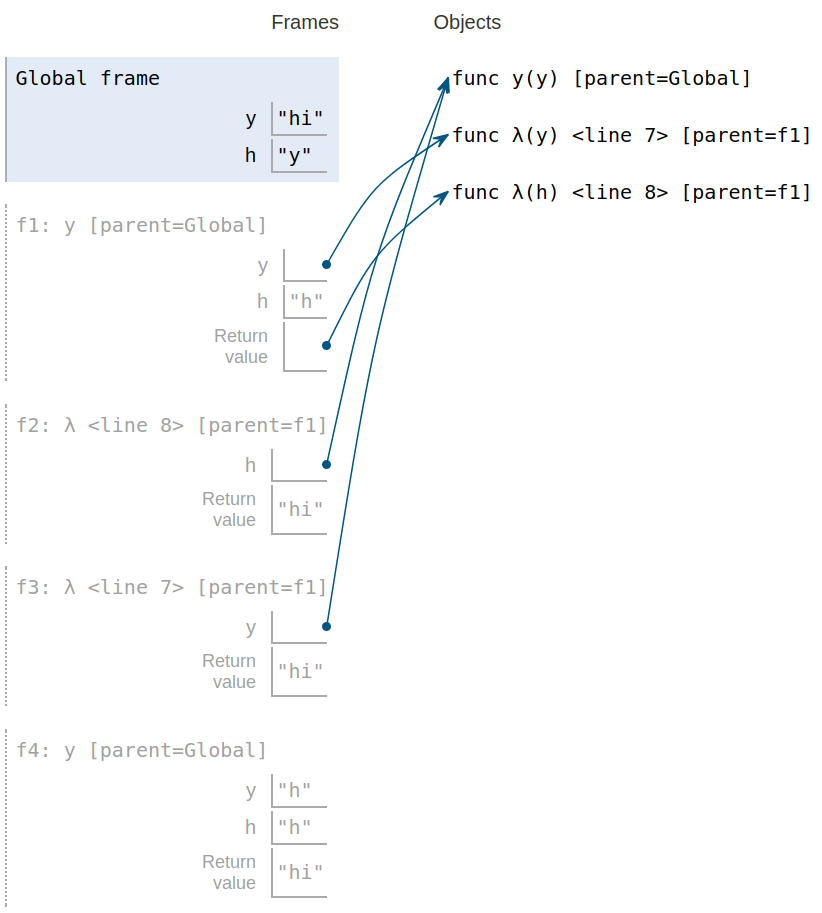
\includegraphics[width=0.7\textwidth]{y.png}
\end{center}
\href{https://www.youtube.com/watch?v=MlRfJaGBeAY&feature=youtu.be}{Video walkthrough}
\end{solution}
